\documentclass[letterpaper]{article}
\usepackage[margin=1in]{geometry}
\usepackage[utf8]{inputenc}
\usepackage{textcomp}
\usepackage{amssymb}
\usepackage{natbib}
\usepackage{graphicx}
\usepackage{gensymb}
\usepackage{amsthm, amsmath, mathtools}
\usepackage[dvipsnames]{xcolor}
\usepackage{enumerate}
\usepackage{mdframed}
\usepackage[most]{tcolorbox}
\usepackage{csquotes}
% https://tex.stackexchange.com/questions/13506/how-to-continue-the-framed-text-box-on-multiple-pages

\tcbuselibrary{theorems}

\newcommand{\R}{\mathbb{R}}
\newcommand{\Z}{\mathbb{Z}}
\newcommand{\N}{\mathbb{N}}
\newcommand{\Q}{\mathbb{Q}}
\newcommand{\C}{\mathbb{C}}
\newcommand{\code}[1]{\texttt{#1}}
\newcommand{\mdiamond}{$\diamondsuit$}
\newcommand{\PowerSet}{\mathcal{P}}
\newcommand{\Mod}[1]{\ (\mathrm{mod}\ #1)}
\DeclareMathOperator{\lcm}{lcm}

%\newtheorem*{theorem}{Theorem}
%\newtheorem*{definition}{Definition}
%\newtheorem*{corollary}{Corollary}
%\newtheorem*{lemma}{Lemma}
\newtheorem*{proposition}{Proposition}


\newtcbtheorem[number within=section]{theorem}{Theorem}
{colback=green!5,colframe=green!35!black,fonttitle=\bfseries}{th}

\newtcbtheorem[number within=section]{definition}{Definition}
{colback=blue!5,colframe=blue!35!black,fonttitle=\bfseries}{def}

\newtcbtheorem[number within=section]{corollary}{Corollary}
{colback=yellow!5,colframe=yellow!35!black,fonttitle=\bfseries}{cor}

\newtcbtheorem[number within=section]{lemma}{Lemma}
{colback=red!5,colframe=red!35!black,fonttitle=\bfseries}{lem}

\newtcbtheorem[number within=section]{example}{Example}
{colback=white!5,colframe=white!35!black,fonttitle=\bfseries}{def}

\newtcbtheorem[number within=section]{note}{Important Note}{
        enhanced,
        sharp corners,
        attach boxed title to top left={
            xshift=-1mm,
            yshift=-5mm,
            yshifttext=-1mm
        },
        top=1.5em,
        colback=white,
        colframe=black,
        fonttitle=\bfseries,
        boxed title style={
            sharp corners,
            size=small,
            colback=red!75!black,
            colframe=red!75!black,
        } 
    }{impnote}
\usepackage[utf8]{inputenc}
\usepackage[english]{babel}
\usepackage{fancyhdr}
\usepackage[hidelinks]{hyperref}

\pagestyle{fancy}
\fancyhf{}
\rhead{Math 170B}
\chead{Friday, April 14, 2023}
\lhead{Lecture 6}
\rfoot{\thepage}

\setlength{\parindent}{0pt}

\begin{document}
\section{Nonlinear Equations \& Bisection Method (Section 3.1)}
Let's consider the problem of finding zeros.

\begin{mdframed}
    (Example.) Suppose we have the functions $\sin(x)$ and $e^x$, and suppose we want to find the values of $x$ such that $\sin(x) - e^x$. Let \[f(x) = \sin(x) - e^x\] so that we can solve for $\sin(x) - e^x = 0$. We want to seek the ``zero'' (i.e., the root) of $f(x)$. 
\end{mdframed}

\subsection{Bisection Method}
The bisection method makes the assumption that $f: \R \mapsto \R$ is \underline{continuous} on an interval $[a, b]$. We want to consider the interval $[a, b]$ so that \[f(a) \cdot f(b) < 0.\] This implies that either $f(x)$ or $f(b)$, but not both, are negative (i.e., $\sgn(f(a)) \neq \sgn(f(b))$).

\begin{center}
    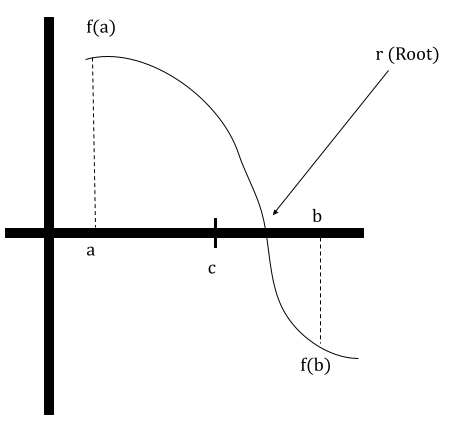
\includegraphics[scale=0.6]{../assets/bisect.png}
\end{center}

Then, we can solve for 
\[c = \frac{b + a}{2} = \frac{a + (b - a)}{2}.\]
$c$ is the midpoint of $a$ and $b$. Then, we let check 
\begin{itemize}
    \item If $f(a) \cdot f(c) < 0$, then we let $b \leftarrow c$ and start with the new interval $[a, b]$. 
    \item Otherwise, $f(b) \cdot f(c) < 0$ and so we let $a \leftarrow c$ and start with the new interval $[a, b]$. 
\end{itemize}
We keep repeating this until the interval becomes sufficiently small. 

\subsection{Algorithm Idea and Stopping Conditions}
Let 
\begin{itemize}
    \item $M$ be the maximum iterations, 
    \item $\delta$ be the interval tolerance ($|b - a| < \delta$), and 
    \item $\epsilon$ be the zero tolerance ($|f(c)| < \epsilon$).
\end{itemize}
The algorithm takes in five inputs: $(M, \delta, \epsilon, a, b)$, where $a$ and $b$ (such that $a \leq b$) represents the interval endpoints (i.e., $[a, b]$).

\begin{algorithm}[H]
    \caption{Bisection Method}
    \label{alg:two}
    \begin{algorithmic}[1]
        \Function{Bisection}{$M, \delta, \epsilon, a, b$}
            \State $u \gets f(a)$
            \State $v \gets f(b)$
            \State $e = b - a$
            \If{$\sgn(u) = \sgn(v)$}
            \State \textbf{Error}
            \EndIf 

            \For{$k \gets 1$ to $M$}
                \State $e \gets e / 2$
                \State $c \gets a + e$
                \State $w \gets f(c)$
                \If{$|e| < \delta$ or $|w| < \epsilon$}
                    \State \textbf{Break}
                \EndIf 

                \If{$\sgn(u) = \sgn(w)$}
                    \State $a \gets c$
                    \State $u \gets w$
                \Else 
                    \State $b \gets c$
                    \State $v \gets w$
                \EndIf 
            \EndFor 

            \State \Return $c$
        \EndFunction
    \end{algorithmic}
\end{algorithm}

\subsection{Tolerances}
We introduces the tolerances, $\delta$ and $\epsilon$, for robustness. 
\begin{itemize}
    \item We might have $|f(c) < \epsilon$ but $|b - a| > \delta$. 
    \begin{center}
        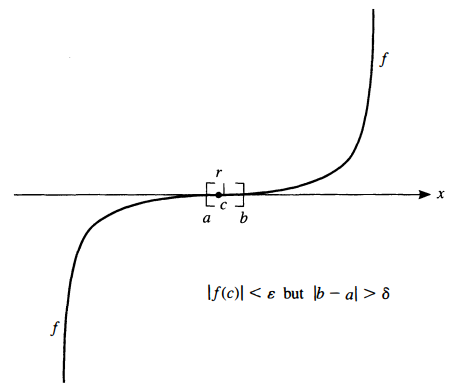
\includegraphics[scale=0.8]{../assets/case1.png}
    \end{center}
    Notice how the graph is flat near the zero. This corresponds to a multiple root, which means the bisection method could have difficulty determining this zero to a high precision.
    \item We also have $|b - a| < \delta$ and $|f(c)| > \epsilon$.
    \begin{center}
        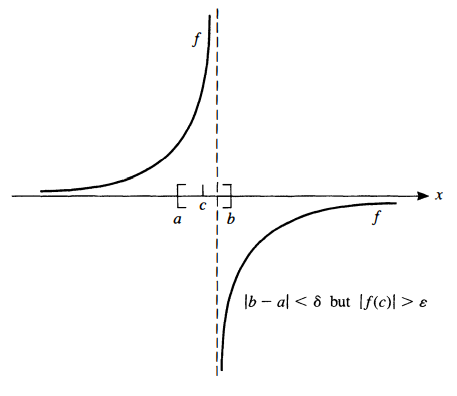
\includegraphics[scale=0.8]{../assets/case2.png}
    \end{center}
    The curve here, which is in the interval $[a, b]$, is not continuous.
\end{itemize}
\textbf{Remark:} From the first point, if we have a function with a double root, then approximation may become less precise or outright impossible. For example, consider $f(x) = (x - 1)^2$, which has a double root of $x = 1$. Because $\forall x \in \R, f(x) \geq 0$, the bisection method cannot be used here.

\subsection{Error Analysis}
Let $I_i = [a_i, b_i]$ be an interval. Then, we essentially have a sequence of intervals, $I_0, I_1, I_2, I_3, \hdots$, where $a_0 \leq a_1 \leq a_2 \leq \hdots \leq b_0$ and $b_0 \geq b_1 \geq b_2 \geq \hdots \geq a_0$.

\begin{verbatim}
    a_m+1      b_m+1
     |---X------|----------|
    a_m        c_m        b_m \end{verbatim}
For $m \geq 0$, We know that $b_{m + 1} - a_{m + 1} = \frac{1}{2}(b_m - a_m)$, so applying it repeatedly gives us 
\[\begin{aligned}
    b_m - a_m &= \frac{1}{2}(b_{m -1} - a_{m - 1}) \\ 
        &= \left(\frac{1}{2}\right)^m (b_0 - a_0)
\end{aligned}.\]
The sequence, $b_m$ and $a_m$, are monotonic and convergent. Because we're constantly dividing the interval by 2, we know that 
\[\lim_{m \mapsto \infty} (b_m - a_m) = \lim_{m \mapsto \infty} \left(\frac{1}{2}\right)^m (b_0 - a_0) = 0.\]
We also know that, as $a$ and $b$ are the left and right endpoints of this interval, both $a$ and $b$ will converge to the root of the equation, $r$, i.e.,
\[\lim_{m \mapsto \infty} a_m = \lim_{m \mapsto \infty} b_m = r.\]
Then, 
\[\lim_{m \mapsto \infty} f(a_m) f(b_m) \leq 0.\] 
This yields \[f(r) f(r) \leq 0 \implies f(r) = 0.\]
Therefore,
\begin{verbatim}
     |-------r--|----------|
    a_m        c_m        b_m \end{verbatim}
In this sense, if at a certain stage in the process we have the interval $I_n$ and the process is now stopped, the root is certain to lie in this interval. However, the best estimate of the root at this stage is not $a_n$ or $b_n$, but the midpoint of the interval, $c_n$. In this sense, the error is then bounded by 
\[|r - c_m| \leq \frac{1}{2}|b_m - a_m|.\]
This gives us the following theorem. 
\begin{theorem}{Bisection Method}{}
    If $I_i = [a_i, b_i]$ is an interval and $I_0, I_1, \hdots, I_n$ denote the intervals in the bisection method, then the limits $\lim_{n \mapsto \infty} a_n$ and $\lim_{n \mapsto \infty} b_n$ exist, are equal, and represent a zero of $f$. If $r = \lim_{n \mapsto \infty} c_n$ and $c_n = \frac{1}{2} (a_n + b_n)$, then 
    \[|r - c_n| \leq \frac{1}{2}|b_n - a_n| = 2^{-(n + 1)}|b_0 - a_0|. \]
\end{theorem}
\begin{mdframed}[nobreak=true]
    (Exercise.) Suppose $[a_0, b_0] = [50, 63]$. How many steps needs to be done using the bisection method to compute a root with relative accuracy of $10^{-12}$? 

    \begin{mdframed}
        We want to seek $|r - c_m| / |r| \leq 10^{-12}$. This means that 
        \[|r - c_m| / 50 \leq 10^{-12}.\]
        (Note that we asked for the \underline{relative} error.) The sufficient condition is \[|r - c_m| / 50 \leq \left(\frac{1}{2}\right)^{m + 1} (b_0 - a_0) / 50 \leq 10^{-12}.\]
        From the theorem, we have 
        \[2^{-(n + 1)}(13 / 50) \leq 10^{-12}.\]
        From there, we can solve for $n$.
    \end{mdframed}
\end{mdframed}


\end{document}